% $Id$
% Author:	Daniel Bosk <daniel.bosk@miun.se>
\documentclass[a4paper]{miunlett}
\usepackage[utf8]{inputenc}
\usepackage[swedish]{babel}
\usepackage{pdfpages}
\usepackage[today,nofancy]{svninfo}

\svnInfo $Id$

% the following settings can be put into ~/texmf/miunlett.conf
% and thus save yourself from rewriting them for all your letters.
\signature{Daniel Bosk\\
	Universitetsadjunkt i datateknik\\
	Kursansvarig
}
\name{Daniel Bosk}
\telephone{060-14\,8709}
\email{daniel.bosk@miun.se}
\institute{Mittuniversitetet}
\address{
	Daniel Bosk\\
	Rum L433\\
	Holmgatan 10\\
	851\,70 Sundsvall
}

\date{Sundsvall, den 7 augusti 2012}

\begin{document}
	\begin{letter}{
		Studenter antagna till\\
		DT001G Informationsteknologi grundkurs
	}
		\opening{Hej,}

		jag är glad att få hälsa dig välkommen till kursen \emph{DT001G 
		Informationsteknologi grundkurs}.

		Kursen kommer att inledas med en introduktionsföreläsning den 3 september 
		kl 15 i Adobe Connect-rummet på adressen
		\begin{center}
			\url{https://connect.sunet.se/miun-itgrund/}.
		\end{center}
		Du behöver fungerande headset och webbkamera.

		Universitetet tillämpar akademisk kvart, vilket innebär att föreläsningen 
		börjar kl 15.15, men logga in 10 minuter tidigare för att se att din 
		utrustning fungerar och för att förändra eventuella inställningar.
		Direkt när du kommer in i Connect klickar du på \emph{Meeting} och väljer 
		\emph{Audio Setup Wizard} i menyn.
		Följ den guiden för att testa och ställa in ditt headset och därefter 
		testar du att dela din webbkamera för att se att den fungerar.

		Till kursstart är det också bra om du införskaffat kurslitteraturen, denna 
		anges i kursplanen som finns bifogad, på så vis undviker du att halka 
		efter.
		Detta är viktigt eftersom att det vid universitetet kan vara högre 
		studietempo än du tidigare erfarit.

		Du kommer att få tillgång till kursen via universitetets lärplattform, 
		i vilken kursen kommer att ges.
		All information kommer att finnas tillgänglig där.


		\closing{Vänligen,}

		\encl{Kursplanen för DT001G Informationsteknologi grundkurs.}

		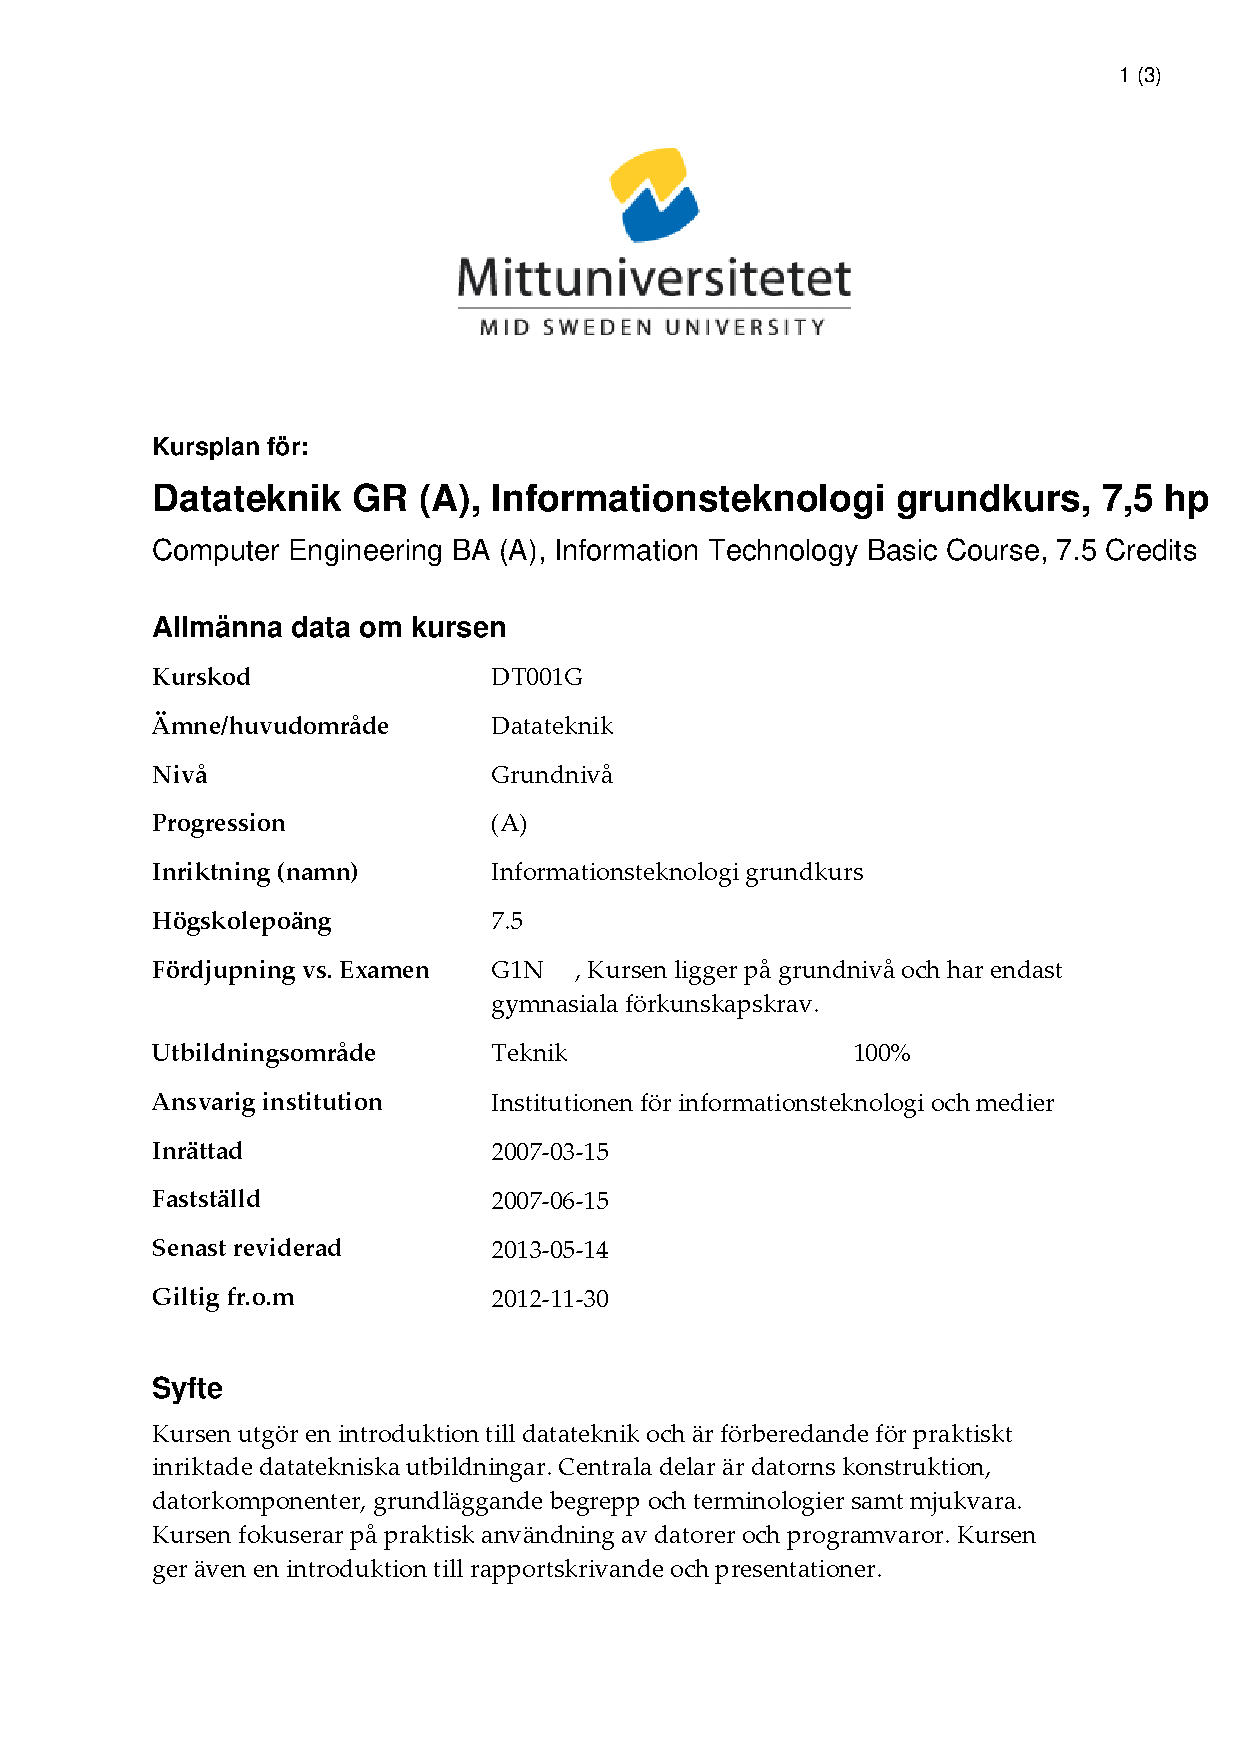
\includepdf[pages=-]{kursplan.pdf}
	\end{letter}
\end{document}
